% !TEX root = main.tex
\section{Ethernet}
Se encuentra entre el \textit{enlace de datos} y \textit{capa fisica}. 
\subsection{Subcapa MAC}
La subcapa MAC de Ethernet tiene dos tareas principales:
\begin{enumerate}
\item encapsulamiento de datos: delimitación de tramas, direccionamiento y detección de errores
\item control de acceso al medio: control de la ubicación y la remoción de tramas en los medios, recuperación de medios.
\end{enumerate}

\begin{figure}[h!]
    \centering
    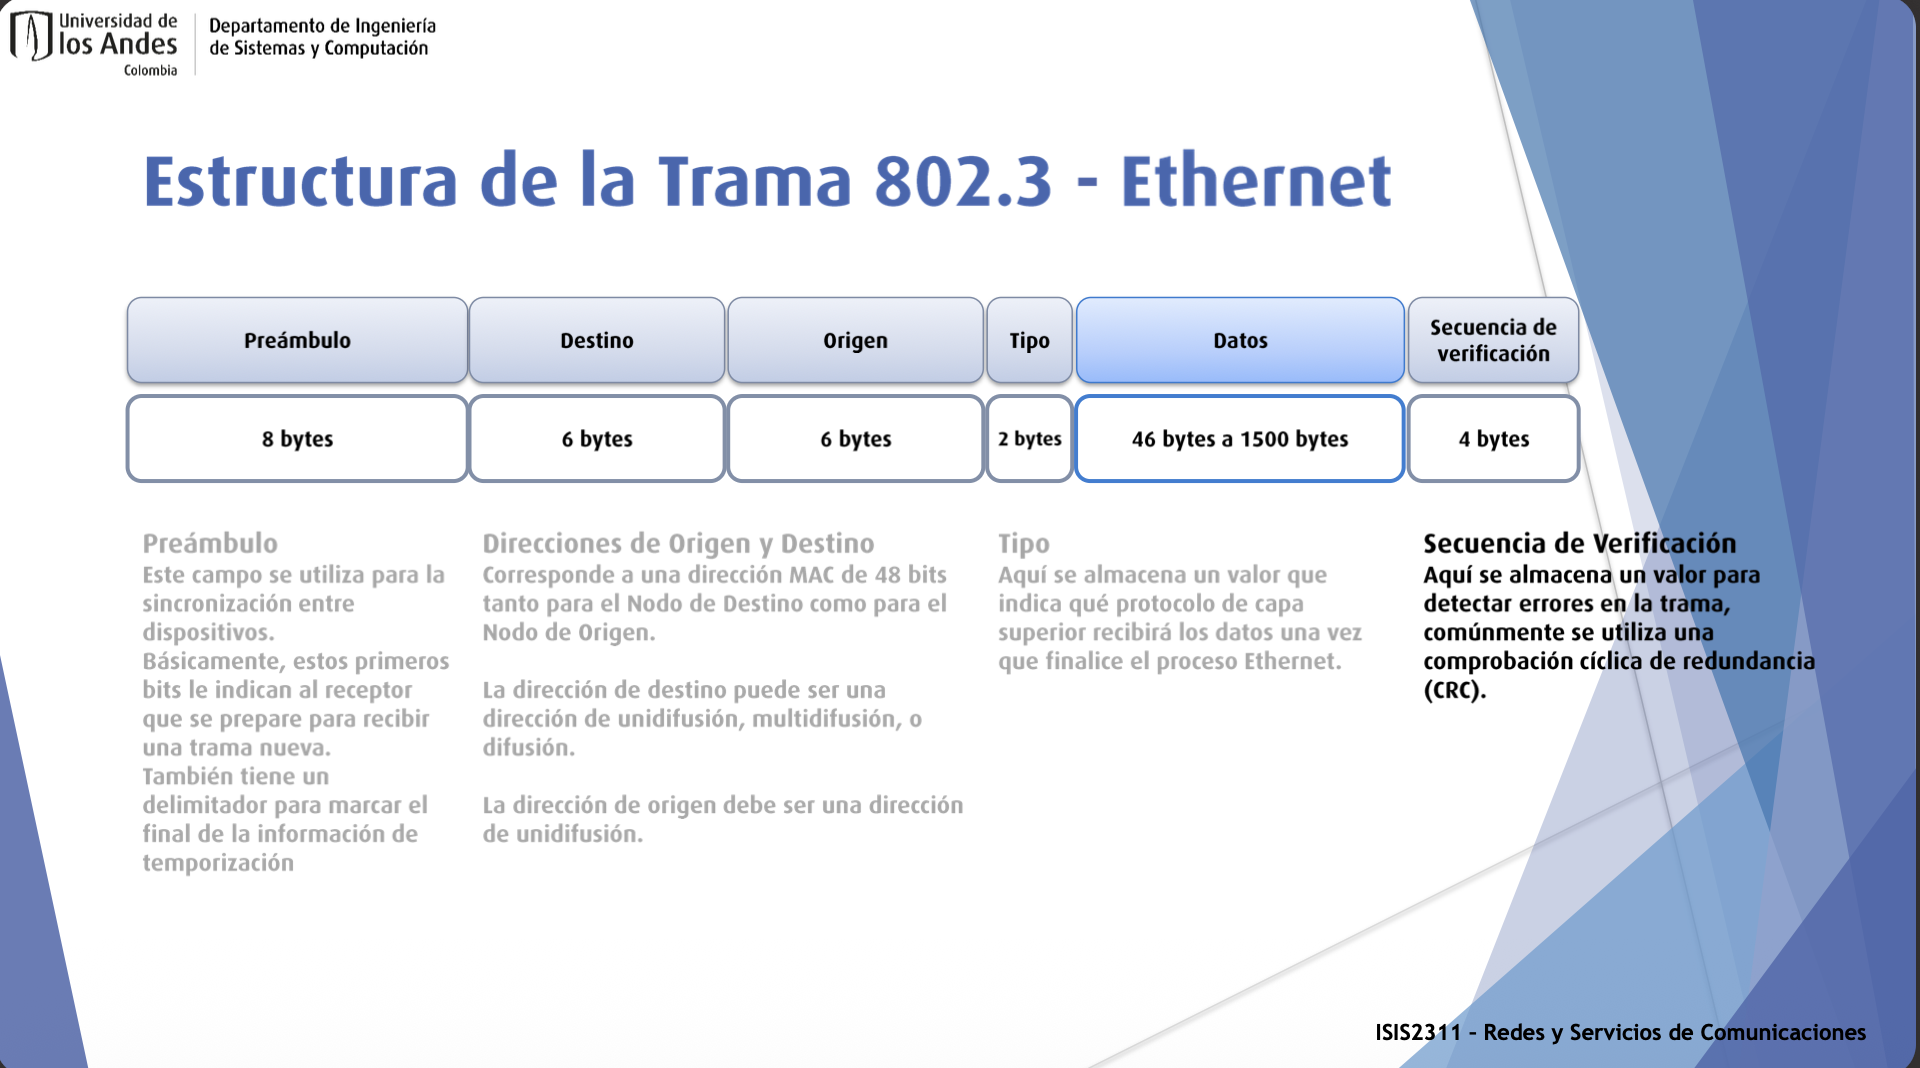
\includegraphics[width=0.5\textwidth]{estructuratramaethernet}
    \label{fig:estructuratramaethernet}
\end{figure}

En la dirección MAC de Ethernet, la \textit{IEEE} asigna al provedor un código de 3 bytes (24 bits) llamado "identificador único de organización".
Todas las direcciones MAC asignadas a una NIC Ethernet deben utilizar el OUI que se le asignó su proveedor. Todas las direcciones MAC con el mismo OUI deben tener asignado un valor único en los tres últimos bytes.

\begin{figure}[h!]
    \centering
    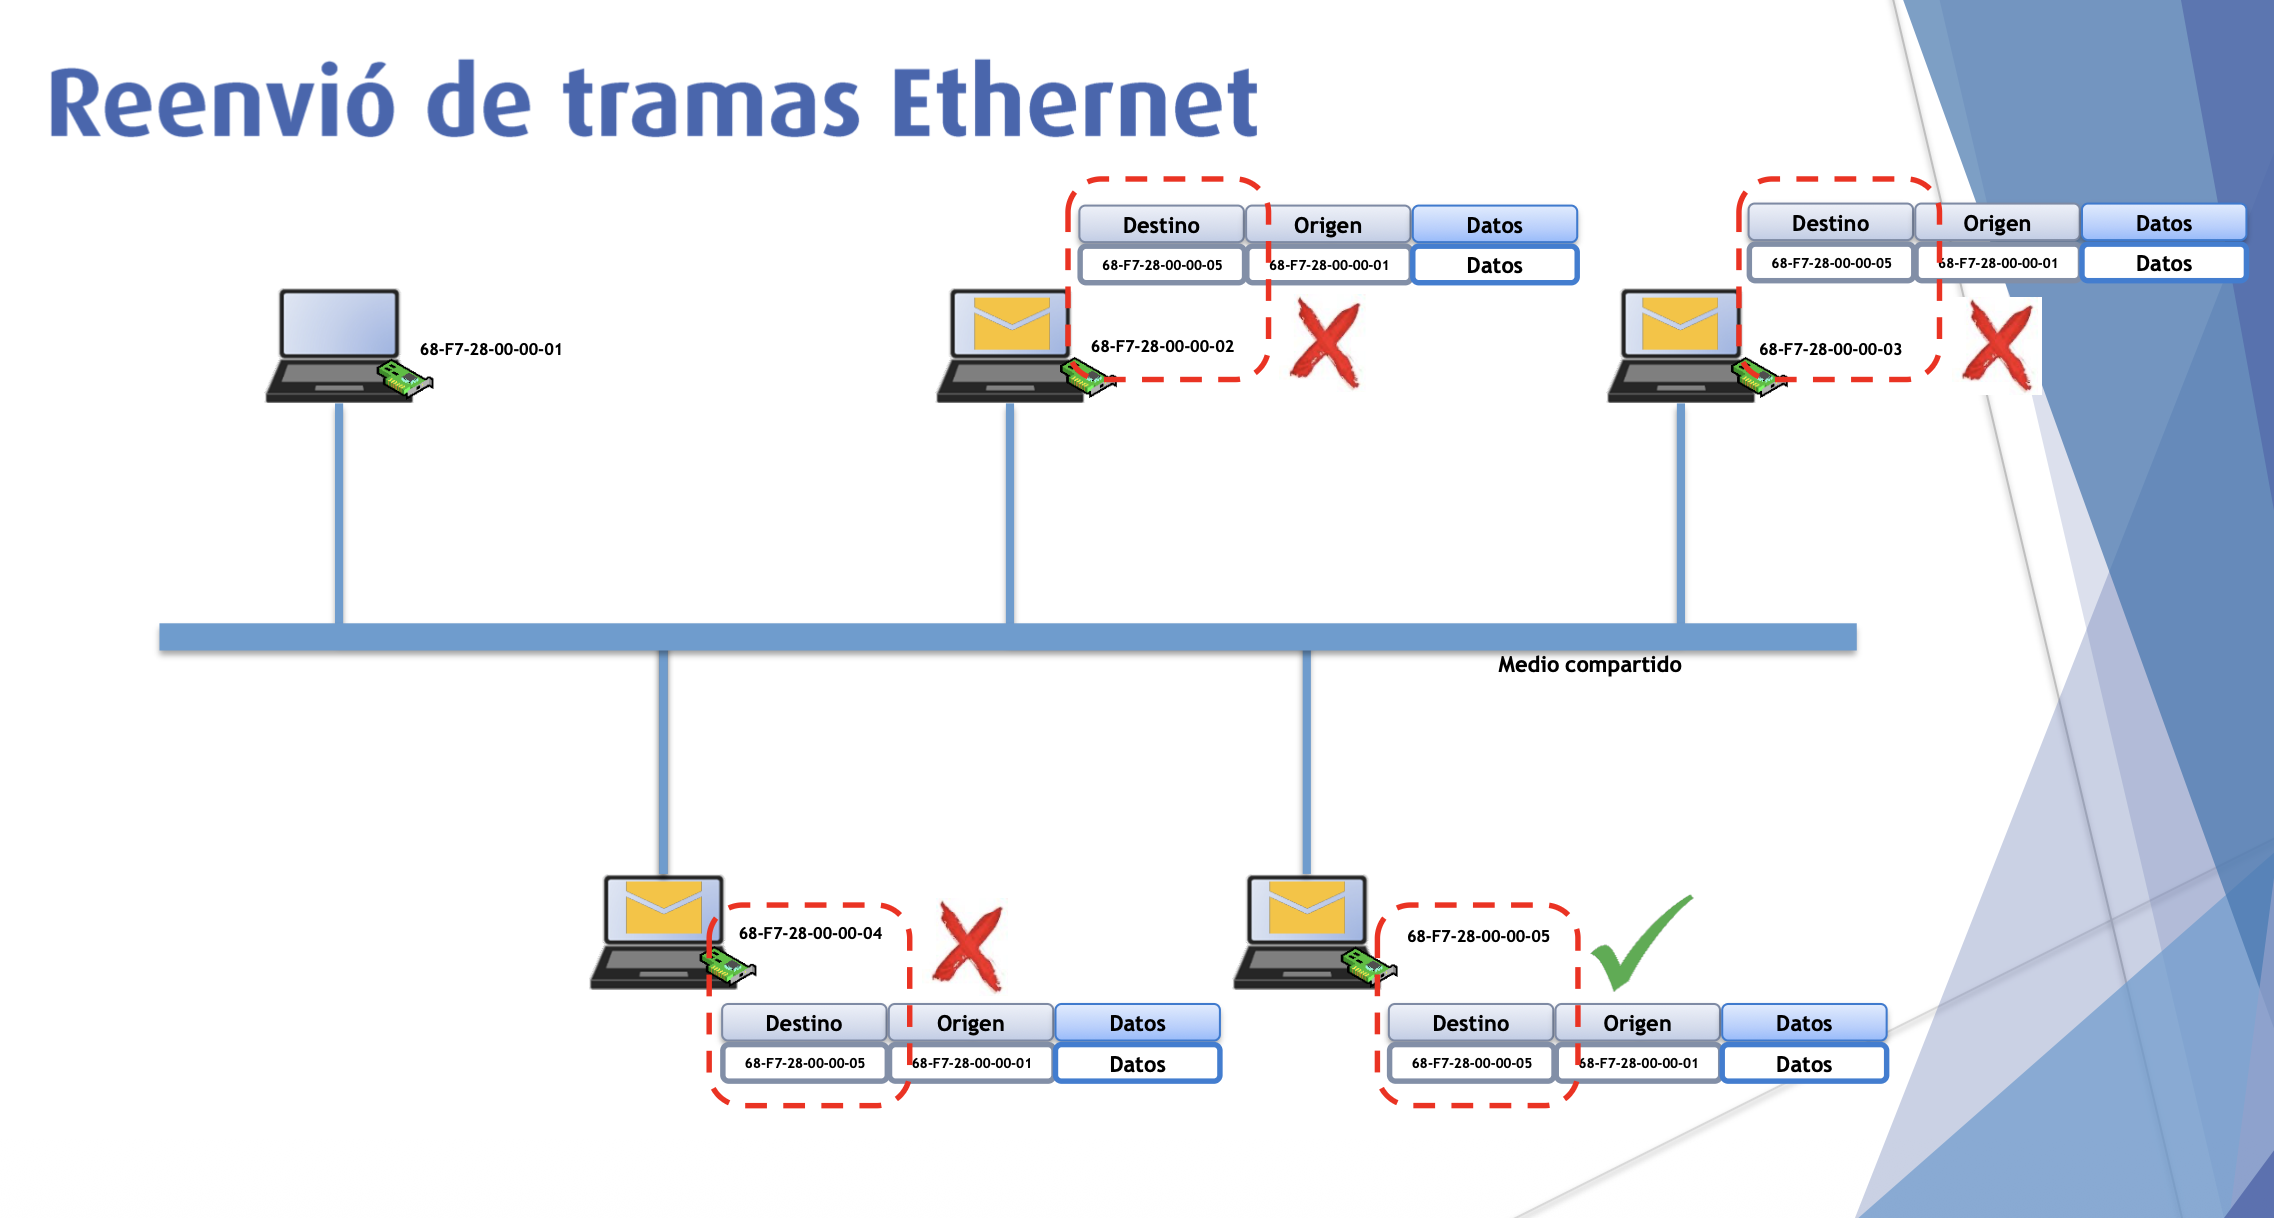
\includegraphics[width=0.5\textwidth]{reenviotramas}
    \label{fig:reenviotramas}
\end{figure}


\subsection{Address Resolution Protocol(ARP)}
es el componente de red encargado de traducir una dirección IP a una dirección física (MAC).
